%%%%%%%%%%%%%%%%%%%%%%%%%%%%%%%%%%%%%%%%%%%%%%%%%%%%%%%%%%
%
% Vzor pro sazbu kvalifikační práce
%
% Západočeská univerzita v Plzni
% Fakulta aplikovaných věd
% Katedra informatiky a výpočetní techniky
%
% Petr Lobaz, lobaz@kiv.zcu.cz, 2016/03/14
%
%%%%%%%%%%%%%%%%%%%%%%%%%%%%%%%%%%%%%%%%%%%%%%%%%%%%%%%%%%

% Možné jazyky práce: czech, english
% Možné typy práce: BP (bakalářská), DP (diplomová)
\documentclass[czech,BP]{thesiskiv}

% Definujte údaje pro vstupní strany
%
% Jméno a příjmení; kvůli textu prohlášení určete, 
% zda jde o mužské, nebo ženské jméno.
\author{Kateřina Kratochvílová}
\declarationfemale

%alternativa: 
%\declarationfemale

% Název práce
\title{Automatická anotace\\obrázků}

\thanktext{Ráda bych poděkovala Ing. Ladislavu Lencovi, Ph.D. za cenné rady, věcné připomínky, trpělivost a ochotu, kterou mi v průběhu zpracování této práce věnoval.}
% 
% Texty abstraktů (anglicky, česky)
%
\abstracttexten{This Bachelor thesis focuses on the automatic image annotation (AIA). The purpose is to verify chosen functions and to try to find their improvements. One of the chosen methods is the Joint Equal Contribution and its modification where the transportation of keywords was changed. Another included method is the Patterns of Oriented Edge Magnitudes method and an implementation of its extensions including color and texture of the image. These methods are described in the theoretical part and then implemented in the practical part. Achieved results are compared to literature in the conclusion. Testing run is done on data sets iaprtc12 and ESP.}

\abstracttextcz{Bakalářská práce se zabývá automatickou anotací obrázků (AIA). Cílem práce je prověřit funkčnost vybraných metod z literatury a pokusit se o jejich vylepšení. V práci byla vyzkoušena metoda Joint Equal Contribution (JEC) a její modifikace, kde bylo pozměněno přenášení klíčových slov. Dále byla otestována metoda Patterns of Oriented Edge Magnitudes (POEM) a implementováno její rozšíření zahrnující barvu i texturu. Metody jsou v teoretické části rozebrány a následně byly implementovány. V konečné fázi byly dosažené výsledky porovnány s literaturou. Testování probíhalo na datasetech iaprtc12 a ESP. 
}

% Na titulní stranu a do textu prohlášení se automaticky vkládá 
% aktuální rok, resp. datum. Můžete je změnit:
%\titlepageyear{2016}
%\declarationdate{1. března 2016}

% Ve zvláštních případech je možné ovlivnit i ostatní texty:
%
%\university{Západočeská univerzita v Plzni}
%\faculty{Fakulta aplikovaných věd}
%\department{Katedra informatiky a výpočetní techniky}
%\subject{Bakalářská práce}
%\titlepagetown{Plzeň}
%\declarationtown{Plzni}

%%%%%%%%%%%%%%%%%%%%%%%%%%%%%%%%%%%%%%%%%%%%%%%%%%%%%%%%%%
%
% DODATEČNÉ BALÍČKY PRO SAZBU
% Jejich užívání či neužívání záleží na libovůli autora 
% práce
%
%%%%%%%%%%%%%%%%%%%%%%%%%%%%%%%%%%%%%%%%%%%%%%%%%%%%%%%%%%

% Zařadit literaturu do obsahu
\usepackage[nottoc,notlot,notlof]{tocbibind}

% Umožňuje vkládání obrázků
\usepackage[pdftex]{graphicx}

% import kvuli vkladani svg, import
\usepackage{graphicx, import}

% tabulky, viceradkove bunky 
\usepackage{multirow}

%barva u tabulek%
\usepackage[table]{xcolor}

%popisky u tabulek
\usepackage{caption}

%hezke cisla v textu%
\usepackage{siunitx}

%seznam u zkratek%
\usepackage{scrextend}

%vicesloupcova sazba%
\usepackage{multicol}

%list
\usepackage{enumitem}

% Odkazy v PDF jsou aktivní; navíc se automaticky vkládá
% balíček 'url', který umožňuje např. dělení slov
% uvnitř URL
\usepackage[pdftex]{hyperref}
\hypersetup{colorlinks=true,
  unicode=true,
  linkcolor=black,
  citecolor=black,
  urlcolor=black,
  bookmarksopen=true}

% matematicke rovnice %
\usepackage{amsmath}
\usepackage{fancyhdr}
\usepackage{float}
% Při používání citačního stylu csplainnatkiv
% (odvozen z csplainnat, http://repo.or.cz/w/csplainnat.git)
% lze snadno modifikovat vzhled citací v textu
\usepackage[numbers,sort&compress]{natbib}

%%%%%%%%%%%%%%%%%%%%%%%%%%%%%%%%%%%%%%%%%%%%%%%%%%%%%%%%%%
%
% VLASTNÍ TEXT PRÁCE
%
%%%%%%%%%%%%%%%%%%%%%%%%%%%%%%%%%%%%%%%%%%%%%%%%%%%%%%%%%%
\begin{document}
%
\maketitle
%\thispagestyle{empty}
%\tableofcontents
\tableofcontents
\addtocontents{toc}{\protect\thispagestyle{empty}}
\thispagestyle{empty}


\chapter{Úvod}
\setcounter{page}{1}
\par V dnešní době, kdy je svět přesycen obrázky v digitální podobě, není vůbec snadné nalézt obrázek zobrazující požadovaný obsah. Naneštěstí počítače nedokáží vnímat obraz jako lidé, vnímají totiž obrazy jako sérii binárních informací. Přitom počítače a jejich práce s obrazy by se dala využít v mnoha oborech jako je lékařství nebo doprava. Na základě toho vyplouvá na povrch problém jak spravovat digitální obrázky a efektivně mezi nimi vyhledávat. Prostřednictvím klíčových slov přiřazených k obrázkům se dá problém vyhledávání zjednodušit. Přiřazení klíčových slov probíhá pomocí procesu automatické anotace obrázků. Klíčová slova přiřazená k obrázku by měla vyjadřovat jeho obsah (například les, strom). Při reálném použití můžeme ovšem narazit na problém při zadávání abstraktních slov, například šťastná rodina.  

\par Pro automatickou anotaci obrázků se používá strojové učení. Anotaci můžeme rozdělit na dvě části. V první části získáme klíčové příznaky, ve druhé už je samotná anotace, tedy přidělení klíčových slov. Abychom tento postup mohli provést v praxi, musíme nejdřív klasifikátor natrénovat pomocí trénovací množiny. Trénovací množina je množina obrázků, která již má ke každému obrázku přidána metadata s klíčovými slovy připravenými od lidí. Vybrané obrázky v trénovací množině by měly být různorodé, aby anotace probíhala správně. Pojem automatická anotace obrázků je jednoduše řečeno proces, při kterém jsou k obrázku automaticky přiřazena metada, která obsahují klíčová slova. 

\par Práce se bude zabývat nízkoúrovňovými příznaky, konkrétně barvou a texturou. Ovšem v případě kdy použijeme barevný příznak, ochudíme se o informaci o textuře obrázku. Pro změnu, když použijeme texturový příznak (který pracuje s šedotónovým obrázkem), zanedbáme informaci o barvě. Jako možnost zpřesnění klasifikátoru by se tedy dalo použít jejich zkombinování. Nabízí se několik řešení \cite{DiplomovaBrno}:   

\begin{description}
\item[Vyhodnotit a klasifikovat příznaky odděleně] 
a poté výslednou klasifikaci spojit z několika částí (například Joint Equal Contribution (JEC) \cite{JEC} ). Výhodou tohoto přístupu je zachování vlastností obou původních příznaků. Nevýhodou je náročnější výpočet. Úspěšnost přístupu závisí na způsobu kombinace obou informací.

\item[Vytvoření společného příznaku.] 
Například rozšíření Patterns of Oriented Edge Magnitudes (POEM) na všechny barvené kanály. Musí se však dbát na to, že informace o barvě a textuře se mohou ovliňovat i protichůdně. 
\end{description} 

\par Cílem práce je navrhnout a implementovat software umožňující automatickou anotaci obrázků za použití nízkoúrovňových příznaků, konkrétně barvy, textury a jejich kombinací. Metody budou testovány na standardních datech IAPRTC12 a ESP. Výsledky dosažené použitím jednotlivých příznaků budou porovnány s literaturou a s nově vytvořeným deskriptorem. V konečné fázi se pokusíme o jejich vylepšení.

\chapter{JEC Joint Equal Contribution}
Tato metoda je založena na hypotéze, že podobné obrázky mají podobná klíčová slova. Pomocí metody hledání nejbližších sousedů (dále jen KNN) je nalezeno K nejpodobnějších obrázků. Přičemž klíčová slova od nejbližšího souseda jsou posuzována odlišným způsobem než klíčová slova od K nejbližších sousedů mimo úplně nejbližšího. Metoda je postavena na dvou typech příznaků - barevných a texturových. 
\cite{JEC}

\section{Příznaky}
\par Barva a textura jsou považovány za dva nejdůležitější nízkoúrovňové příznaky pro obrázkovou reprezentaci. Nejběžnější barevné deskriptory jsou barevné histogramy, které jsou často využívány pro porovnávání a indexování obrázků, zejména z důvodu jejich efektivnosti a snadného výpočtu. K~vytvoření texturových příznaků se používají Haarovy a Gaborovy wavelety a to především z důvodu efektivity při vytváření řídkých a zároveň diskriminativních obrázkových rysů. Při snaze omezit vliv předpokladů jednotlivých funkcí a maximalizovat množství získaných informací je použito několik jednoduchých a snadno sestavitelných funkcí. \cite{JEC}

\subsection{Barva}
\par U digitálního obrazu je barva reprezentovaná n-rozměrným vektorem. Jeho velikost a význam jednotlivých složek (tzv. barevných kanálů) zavisí na příslušném barevném prostoru. Počet bitů použitých k uložení, buď celého vektoru nebo jeho jednotlivých složek, se nazývá barevná hloubka (totožně bitová hloubka). Obvykle se můžeme setkat s hodnotami 8, 12, 14 a 16 bitů na kanál. 

\par V použité metodě jsou získány vlastnosti z obrázků ve třech rozdílných barevných prostorech: RGB, HSV a LAB. RGB (Red, Green, Blue) je nejpoužívanější barevný prostor pro zachycení obrázu nebo jeho zobrazení. Oproti tomu HSV (Hue, Saturation and Value) se snaží zachytit barevný model tak, jak ho vnímá lidské oko. Zároveň usiluje o to zůstat jednoduchý pro výpočet. Hue znamená odstín barvy (měří se jako poloha na standardním barevném kole $0^{\circ} - 360^{\circ}$ ), saturation je systost barvy (množství šedi v poměru k odstínu $0 \%$ šedá barva - $100 \%$ plně sytá barva). Value je hodnota jasu nebo také množství bílého světla (relativní světlost nebo tmavost barvy). Některé kombinace hodnot H, S a V mohou dávat nesmyslné výsledky. RGB je závislý na konkrétním zařízení, které nemůže dosáhnout celého rozsahu barev, které vidí lidské oko. Zatímco barevný model LAB je schopen obsáhnout celé viditelné spektrum a navíc je nezávislý na zařízení. L (ve zkratce LAB) značí luminanci (jas dosahuje hodnot 0 - 100, kde 0 je černá a 100 je bílá). Zbylé A a B jsou dvě barvonosné složky, kdy A je ve směru červeno/zeleném a B se pohybuje ve směru modro/žlutém.

\begin{figure}[H]
		\centering
		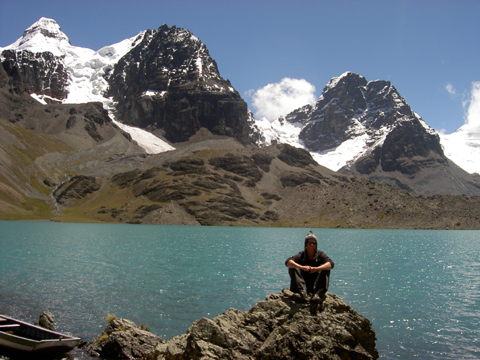
\includegraphics[height=100px]{./img/img_histogram.jpg}	
		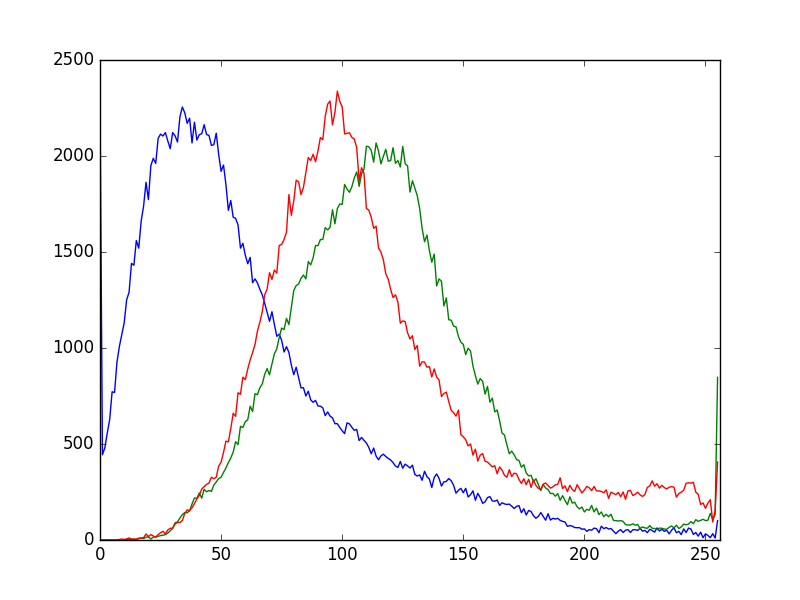
\includegraphics[height=100px]{./img/bgr_histogram.png}	
		\caption{RGB histogram - zastoupení jednotlivých složek v obrázku}
\end{figure}

\begin{figure}[H]
		\centering
		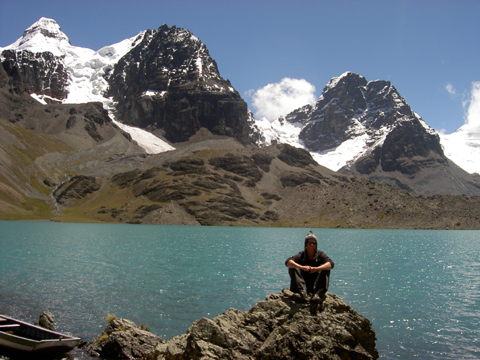
\includegraphics[height=100px]{./img/img_histogram.jpg}
		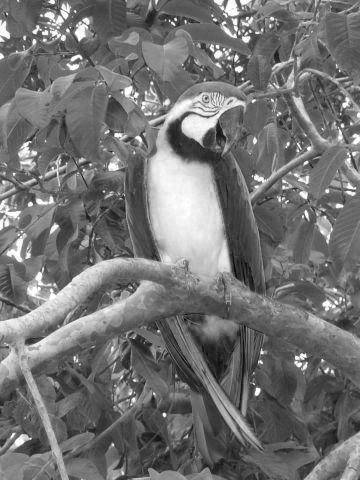
\includegraphics[height=100px]{./img/bgr_r.jpg}
		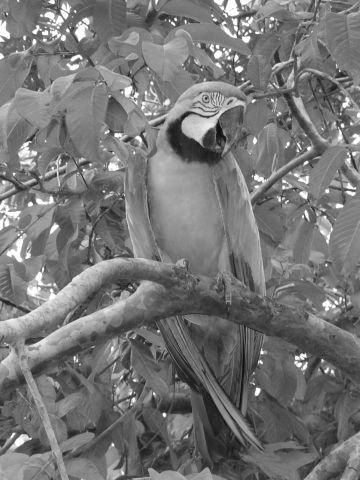
\includegraphics[height=100px]{./img/bgr_g.jpg}
		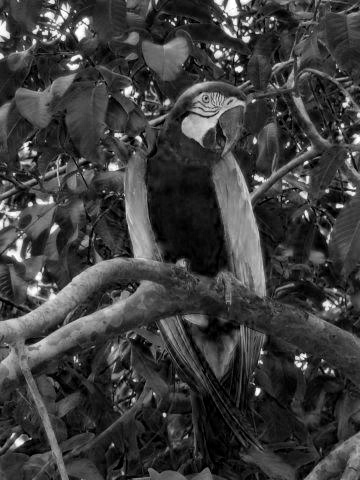
\includegraphics[height=100px]{./img/bgr_b.jpg}	
		\caption{Barevný prostor RGB a jeho jednotlivé složky v pořadí R,~G,~B}
\end{figure}

\begin{figure}[H]
		\centering
		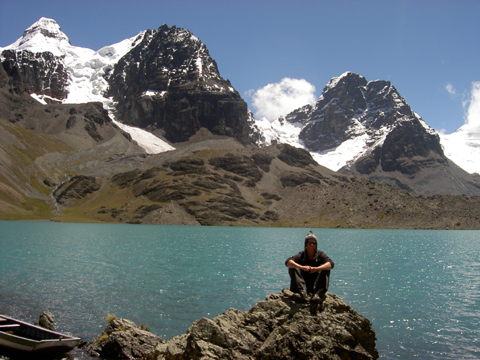
\includegraphics[height=100px]{./img/img_histogram.jpg}
		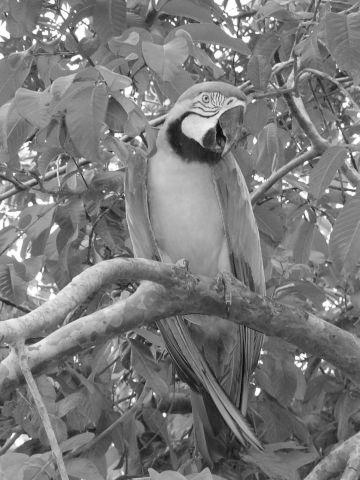
\includegraphics[height=100px]{./img/lab_l.jpg}
		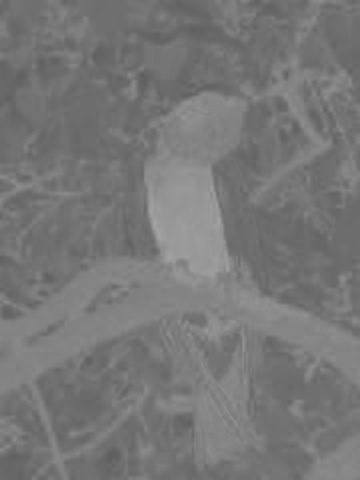
\includegraphics[height=100px]{./img/lab_a.jpg}
		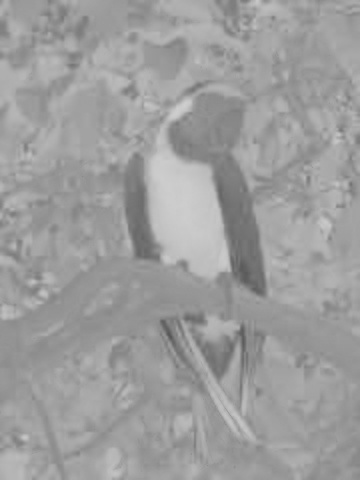
\includegraphics[height=100px]{./img/lab_b.jpg}	
		\caption{Barevný prostor LAB a jeho jednotlivé složky v pořadí L,~A,~B}
\end{figure}

\begin{figure}[H]
		\centering
		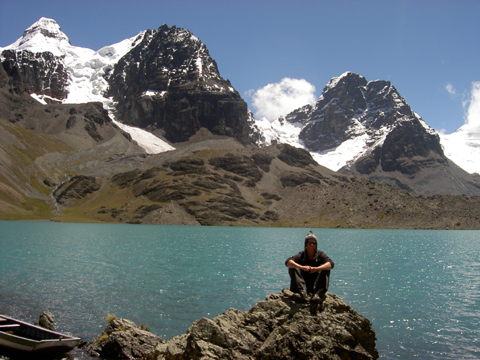
\includegraphics[height=100px]{./img/img_histogram.jpg}
		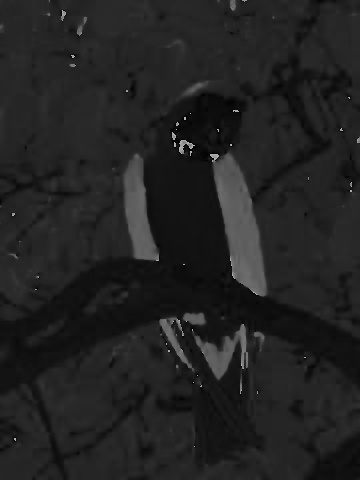
\includegraphics[height=100px]{./img/hsv_h.jpg}
		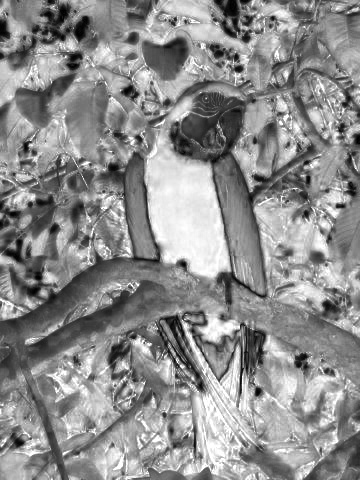
\includegraphics[height=100px]{./img/hsv_s.jpg}
		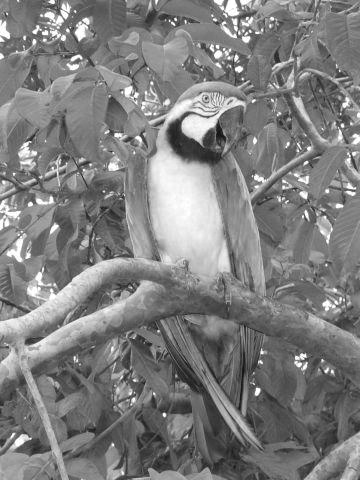
\includegraphics[height=100px]{./img/hsv_v.jpg}	
		\caption{Barevný prostor HSV a jeho jednotlivé složky v pořadí H,~S,~V}
\end{figure}

\par Pro RGB, HSV i LAB je použito 16 binů na kanál histogramu v jejich příslušném barevném prostoru. To znamená, že z každého barevného prostoru vzniknou tři šestnácti prvkové histogramy. Tyto histogramy jsou zřetězeny a následně použity jako reprezentace příslušného barevného prostoru.
 
\par  Algoritmus pro výpočet histogramu jednoho kanálu je následující: Jako první bude připraven vektor nul představující histogram. Při výpočtu histogramu algoritmus prochází postupně jednotlivé hodnoty pixelu kanálu vstupního obrázku. Tato hodnota je vydělena 16. Výsledek určuje pozici (index) hodnoty ve vektoru, která má být inkrementována.

\subsection{Textura}
\par Jako reprezentace textur budou použity Gaborovy a Haarovy vlnky (v originále Gabor a Haar wavelet). 

\subsubsection{Gabor}
\par Gaborův filtr je lineární filtr používaný pro analýzu textury, který zkoumá, zda existuje nějaký specifický frekvenční obsah v obraze ve specifických směrech v lokalizované oblasti kolem pole analýzy. Frekvence a orientace reprezentující Gaborovy filtry je podobná lidskému vnímání a proto je jejich použití zvláště vhodné při reprezentaci textury a detekci hran. V prostoru je 2D Gaborův filtr funkcí Gausova jádra modulovaného sinusouvou rovinnou vlnou. Gaboruv filtr je definován v rovnici~\ref{gabor_complex}.

\begin{figure}[H]
		\centering
		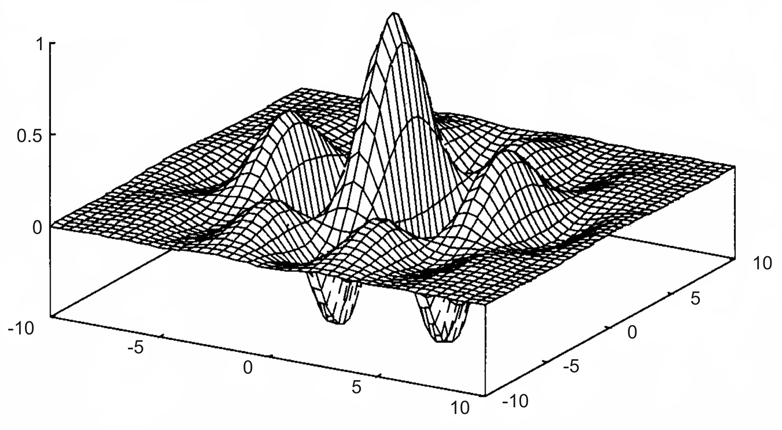
\includegraphics[height=200px]{./img/gabor.png}
		\caption{Gaborova vlnka je tvořena kombinací dvou cosinových funkcí, s rozdílnou frekvencí pro každou osu, a následně jsou vynásobeny dvourozměrnou Gaussovou funkcí \cite{Gabor}.} 					
\end{figure}

\begin{align}
   \label{gabor_complex}  g(x, y; \lambda, \theta, \psi, \sigma,  \gamma) = exp \Bigg( - \frac{{x^2 + \gamma^2 y^2}}{2 \sigma^2} \Bigg) exp \Bigg(i \bigg(2\pi \frac{x}{\lambda} + \psi \bigg)\Bigg)  
\end{align}

\par Gaborovy filtry jsou aplikovány na obrázky stejnou cestou jako běžné filtry. Základ tvoří maska (přesnější termín je konvoluční jádro), která reprezentuje filtr. Maskou je myšleno pole (obyvykle 2D protože se jedná o 2D obrázky) pixelů, ve kterém každý pixel má přiřazenou hodnotu (váhu). Toto pole je přesunuto na každý pixel obrazu a je provedena konvoluční operace. Když je na obrázek aplikován Gaborův filtr, poskytuje nejvyšší odezvu na hranach a místech, kde se textura mění. \cite{Gabor_wordpress}

\par Gaborův filtr reaguje na hrany a změny textury. Když se řekne, že filtr odpovídá na konkrétní funkci, myslí se tím, že podle parametrů reaguje na změny v obraze, které mají určitou frekvenci a orientaci. 

U Gaborova filtru máme několik parametrů, které ovlivňují jeho vlastnosti: 
\paragraph{ksize} -určuje velikost Gabor jádra. Když je ksize (a, b), je získáno jádro velikostí $a \times b$ pixelů. Jako u mnoha jiných konvolučních jader je preferován rozměr čtverce o lichých hranách a to z důvodu umístění středu filtru na pixel. Pří různých ksize se velikost konvolučního jádra mění. 

\paragraph{sigma} -označuje směrodatnou odchylku Gaussovy funkce použitou v Gaborově filtru. Tento parametr kontroluje šířku Gaussovy obálky použité v Gabor jádře.

\paragraph{theta} -je orientace normály na paralelní pruhy Gaborovy funkce. Představuje možná jeden z nejdůležitějších parametrů Gaborova filtru. Theta rozhoduje jakého druhu funkce je tzn. na jaký typ funkce filtr reaguje. Například při nulové thetě bude filtr reagovat pouze na vodorovné příznaky. Proto, abychom získali vlastnosti v různých úhlech obrazu, rozdělíme interval mezi $0^\circ-180^\circ$ na několik stejných částí a vypočítáme Gaborovo jádro pro každou takto získanou hodnotu theta.

\paragraph{lambda} -udává vlnovou délku sinusové funkce ve výše uvedené rovnici.

\paragraph{gamma} -určuje prostorový poměr stran. Kontroluju elipsicitu Gausovy funkce. Když je gamma = 1 je Gauss do kruhu (obalen kruhem)

\paragraph{psí} -je fázový posun (určuje jestli nám vrátí reálnou nebo imaginární část). \\ 

\par Podle \citep{JEC} bude každý obrázek filtrován na třech vlnových délkách a čtyřech orientacích. Výsledkem bude 12 filtrovaných obrázků pro jeden původní obrázek. 


\begin{figure}[H]
	\centering
	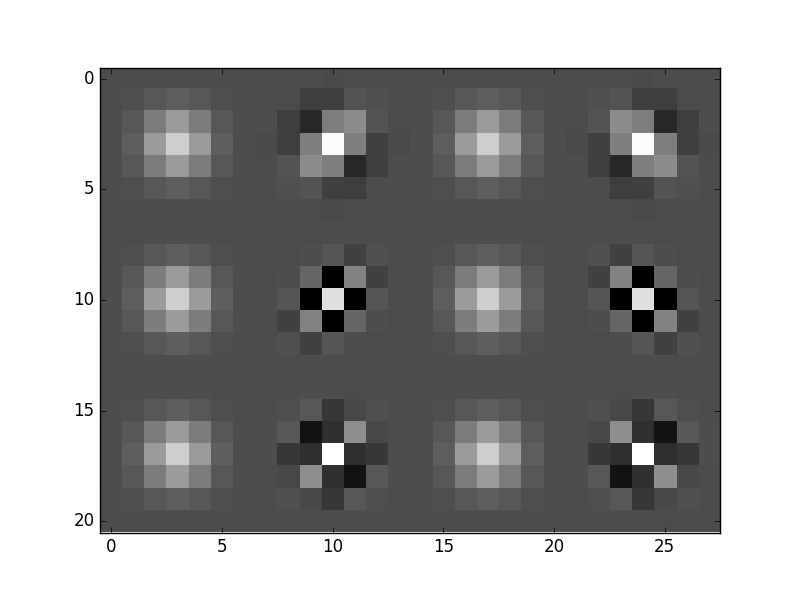
\includegraphics[width=190px]{./img/gabor_filtry.png}
	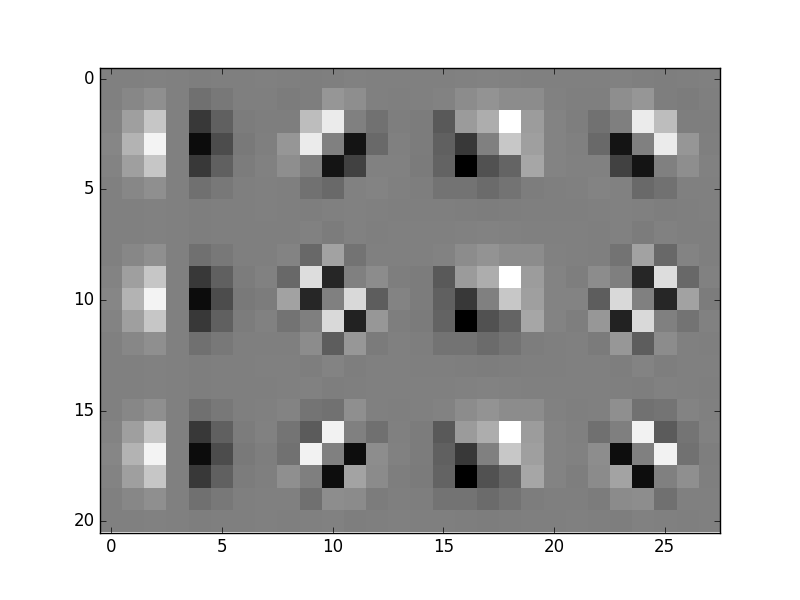
\includegraphics[width=190px]{./img/gabor_filter_imag.png}	
	\caption{Podoba použítých Gaborových filtrů. Vlevo reálná část, vpravo imaginární část.}
	%\label{img:esp_coin}
\end{figure}

\par Po použití filtru na obrázek vzniknou dvě matice, jedna pro reálnou část a jedna pro část imaginární. Prvky matic se vybírají po dvojicích, jeden prvek z reální části a jeden z části imaginární, vždy se stejnými souřadnicemi a je na ně pohlíženo jako na vektory. Pro vzniklé vektory je spočtena jejich velikost, označena jinak jako magnituda. Tato část je opakována pro každý filtr, tedy 12krát.

\par Z každého z dvanácti obrázků bude postaven 16 binový histogram skrze získané magnitudy. Vzniklé histogramy magnitud jsou zřetězeny a označeny jako příznak Gabor. 

\par Druhý příznak zachycující fáze, je označen jako GaborQ. Opět jsou prvky matice vybírány po dvojicích, jeden prvek z reálné části a jeden z části imaginární, vždy se stejnými souřadnicemi. U vzniklých vektorů je tentokrát pohlíženo na velikost úhlu, který svírají s osou x. Jinak se dá tento úhel označit jako fáze.   
\par Vzniklé fáze jsou převedeny na 16 binové histogramy pro každý z dvanácti obrázků a v konečné fázi zřetězeny.


\subsubsection{Haar}
\par Haarova vlnka je nejjednodušší vlnka, jejíž výhodou je především rychlý výpočet. Vlnka je realizována dvěma jednotkovými skoky, z čehož vzniknou dva obdelníkové pulzy s přechodem od kladného k zápornému. 

\begin{figure}[H]
    \centering
    %\def\svgwidth{\columnwidth}
    \def\svgwidth{200px}
    \import{img/}{haar_wavelet.pdf_tex} 
    \caption{Haarova vlnka.}
    %\input{soucet_vektoru.pdf_tex}
\end{figure} 

Předpis Haarovy vlnky:

\begin{displaymath} 
	\label{haar} 
		    \psi(x) = \left\{ \begin{array}{r@{\quad}c}
    		1 & 0 \leq x < \frac{1}{2}, \\
    		-1 & \frac{1}{2} \leq x < 1, \\ 
    		0 & jinde. \\  \end{array} \right. 
\end{displaymath} 
\vspace{1cm}

%Haarovi vlnové filtry reprezentují obrázek jako množinu oblastí a získavají průměrnou intenzitu z nejbližších sousedních oblastí. %Jsou schopny extrahovat charakteristiky daných vlastností obrázku jako jsou například hrany nebo změny v textuře. 

\par Haarovy vlnové filtry jsou schopny extrahovat charakteristiky daných vlastností obrázku, jako jsou například hrany nebo změny v textuře.  Při zpracovávání průměrné intenzity oblastí je snížena citlivost na šum a změny jasu. Velká množina Haarových filtrů se skládá z filtrů s různým počtem obdelníkových oblastí a s různými orientacemi vzhledem k vyzdvižení různorodých texturových informací obrázku. Haarův vlnový filtr nabízí jednoduché a efektivní získávání informací z obrázků.
\par Základní Haarův vlnový filtr bere v potaz přilehlé obdelníkové oblasti v dané části obrázku a počítá rozdíl intenzit mezi nimi. 
 
\par Podle \citep{JEC} bude Haarova vlnka generovat konvoluční blok s Haarovými filtry na třech rozdílných orientacíh (horizontální, diagonální a vertikální) použité na obrázky čtyř různých velikostí. Různé velikosti obrázku jsou získány postupným zmenšováním podle vzorce \ref{Haar_factor_resize}. Vzorec je přízpůsoben, aby v případě nejmenšího rozměru obrázku byla velikost menší ze stran 64 pixelů. 

\par Je definovan \textit{factor\_resize} jako faktor změny velikosti obrázku, \textit{min\_size} jako velikost menší strany obrázku a \textit{scales} jako požadovaný počet různých velikostí obrázků. 

\begin{align}
   \label{Haar_factor_resize} factor\_resize = \Bigg(\frac{64}{min\_size}\Bigg)^{\frac{1}{scales}}   
\end{align}

\par Při velikosti vstupního obrázku $480 \times 360$ pixelů, vyjde faktor změny velikosti $0.562$. Další rozměry obrázku tedy budou $270 \times 202$, $152 \times 114 $ a $85 \times 64$ pixelů.


\vspace{0.5cm}
\noindent Haarovy filtry: 
\definecolor{ashgrey}{rgb}{0.7,0.75,0.71} 

\begin{multicols}{3}
	\begin{center}
		\begin{tabular}{ | c | c | }
    		\hline
    		\cellcolor{ashgrey!50}-1 & \cellcolor{ashgrey!50}-1 \\ \hline
    		1 & 1 \\ 
    		\hline
    	\end{tabular}
    	\vspace{0.5cm}
    	\par Vertikální
	\end{center}
	\begin{center}
		\begin{tabular}{ | c | c | }
    		\hline
    		\cellcolor{ashgrey!50}-1 & 1 \\ \hline
    		\cellcolor{ashgrey!50}-1 & 1 \\ 
    		\hline
    	\end{tabular}
		\vspace{0.5cm}
    	\par Horizontální
	\end{center} 	
	\begin{center}
		\begin{tabular}{ | c | c | }
    		\hline
    		\cellcolor{ashgrey!50}-1 & 1 \\ \hline
    		1 & \cellcolor{ashgrey!50}-1 \\ 
    		\hline
    	\end{tabular}
		\vspace{0.5cm}
    	\par Diagonální
	\end{center} 	
\end{multicols}

\par Z článku \cite{JEC} není přesně zřejmé jak autoři příznak vypočítali. Tato práce je zaměřena na dva možné postupy. Po aplikaci filtru kombinacemi velikostí a orientací vždy vznikne 12 matic. 
\par První možností je výsledné matice postupně převést na 16ti prvkové vektory. Tímto vyjde 12 šestnácti prvkových vektorů pro jeden obrázek, které jsou v konečné fázi zřetězeny. 
\par Další možností je udělat z každé z výslednách matic průměr. Výsledným vektorem bude v tomto případě 12ti prvkový vektor průměrů. 

\par Příznak HaarQ používá stejný filtr jako Haar s tím rozdílem, že po aplikaci filtru jsou přepočítány jednotlivé prvky matice. Při hodnotě menší než 0 je prvek nahrazen -1, a při hodnotě větší než 0 je nahrazen 1. Z výsledné matice je utvořen její průměr. Tím opět pro jeden obrázek vznikne 12ti prvkový vektor průměrů.   

\section{Vzdálenosti}
\par Pro výpočet vzdáleností vektorů se používají následující metody Kullaback-Leibler divergence (dále jen KL - divergence), $\chi^2$ statistika, L1 - vzdálenost a L2 - vzdálenost. Na RGB a HSV je nejlépší použít L1 zatímco pro LAB je nejvhodnější KL - divergence. 

Problém s KL - divergencí nastává pouze tehdy, když se histogramy neshodují v nulách. To plyne z předpokladu pro fungování tohoto vzorce: Když je $Q(i) = 0$ tak zároveň musí být i $P(i) = 0$. \\

Kullaback-Leibler divergence:
\begin{align}
   \label{kl}  D_{KL} (P || Q) = \sum_{i} P(i) \log_e \bigg({\frac{P(i)}{Q(i)}} \bigg) 
\end{align}

L1 (jinak označováno jako Manhattan):
\begin{align}
   \label{L1} L_1 = \sum_{i=1}^{N} |x_i - y_i|  
\end{align}

L2 (jinak označováno jako Euklidovská vzdálenost)
\begin{align}
   \label{L2} L_2 = \sqrt{\sum_{i=1}^{N} (x_i - y_i)^2}  
\end{align}
 
\section{Kombinace vzdáleností}
\par Nejjednodušším přístupem ke zkombinování vzdáleností od různých deskriptorů je, aby jednotlivé vzdálenosti přispívaly rovnoceně. Z tohoto důvodu je potřeba vzdálenosti přeškálovat na jednotné měřítko.

\par $I_i$ představuje $i$-tý obrázek s $N$ příznaky. $d_{(i,j)}^k$ představuje vzdálenosti mezi příznaky $f_i^k$ a $f_j^k$. Při snaze zkombinovat všechny vzdálenosti příznaků mezi obrázky $I_i$ a $I_j$, tedy $d_{(i,j)}^k$ , $k=1, ..., N$  je třeba dbát na to, že v praxi nevyjdou tak, aby měly stejný poměr na výsledku. Z tohoto důvodu, před zkombinování vzdáleností, je třeba je normalizovat do jednotné formy. Na základě získaných maximálních a minimálních hodnot pro každý příznak jsou vzdálenosti přeškálovány na interval od 0 do 1. Jestliže je přeškálována vzdálenost označena jako ${\tilde{d}_{(i,j)}^k}$ následně může být kompletní vzdálenost mezi obrázky $I_i$ a $I_j$ označena jako \eqref{jec} Joint Equal Contribution (JEC).  

\begin{align}
   \label{jec} JEC = \sum_{k=1}^N\frac{\tilde{d}_{(i,j)}^k}{N}
\end{align}

\section{Přenesení klíčových slov}
\subsection{Originální algoritmus pro přenesení klíčových slov metody JEC}
\par Pro přenesení klíčových slov je použita metoda, kdy je přeneseno $n$ klíčových slov k dotazovanému obrázku $\tilde{I}$ od K nejbližších sousedů z trénovací sady. Je nadefinováno $I_{i}, i = 1, ..., K$, těchto K nejbližší sousedů je seřazeno podle vzrůstající vzdálenosti (tzn. že $I_{1} $ je nejvíce podobný obrázek). Počet klíčových slov k danému $I_{i}$ je označen jako $|I_{i}|$. Dále jsou popsány jednotlivé kroky alogoritmu na přenesení klíčových slov.
\begin{enumerate}
	\item Klíčová slova z $I_{1}$ jsou seřazena podle jejich frekvence výskytu v trénovací sadě.
	\item Ze všech $|I_{1}|$ klíčových slov z $I_{1}$ je přeneseno $n$ nejvíce vyskytujících se v trénovací sadě k dotazovanému $\tilde{I}$. Když $|I_{1}| < n$ algoritmus pokračuje na krok 3. 
	\item Klíčová slova sousedů od $I_{2}$ do $I_{K}$ jsou seřazena podle dvou faktorů
	\begin{enumerate}
		\item výskytu v trénovací sadě s klíčovými slovy přenesenými v kroku~2
		\item místní frekvence (tj. jak často se vyskytují jako klíčová slova u obrázků $I_{2}$ až $I_{K}$). Jsou vybrána nejčetnější $n-|I_{1}|$ klíčových slov převedených do $\tilde{I}$.
	\end{enumerate}
\end{enumerate}

\par Tento algoritmus pro přenos klíčových slov je poněkud odlišný od algoritmů, které se běžně používají. Jeden z běžně užívaných funguje na principu, že klíčová slova jsou vybrána od všech sousedů (se všemi sousedy je zacházeno stejně bez ohledu na to, jak jsou danému obrázku podobní). Jiný užívaný algoritmus k sousedům přistupuje váženě (každý soused má jinou váhu) a to na základě jejich vzdálenosti od testovaného obrázku. Podle testů v článku \citep{JEC}, přinášely tyto přímé postupy horší výsledky v porování s použitým dvoufaktorovým algoritmem pro přenos klíčových slov. \\
 
\subsection{Dynamické přenesení klíčových slov pomocí prahování}
\par Pro přenesení klíčových slov lze použít algoritmus, kdy přeneseme pouze ta klíčová slova, která svými výskyty přesahují předepsaný práh. Je definováno $total\_keywords$ jako počet všech klíčových slov i s jejich redundantními výskyty, $frequence\_keyword$ - počet výskytů daného slova v k nejbližších sousedech a $count\_keywords$ jako počet jedinečných klíčových slov (bez redundantních výskytů).  

\par Práh \eqref{prah} je vyčíslen jako jedna děleno počtem všech klíčových slov i s jejich redundantními výskyty - 1. Následuje výpočet váhy pro dané klíčové slovo \eqref{vaha_klicoveho_slova}, který probíhá jako počet výskytů daného slova děleno počet všech klíčových slov i s jejich redundantními výskyty. Pokud je tato hodnota vyšší než práh, je klíčové slovo přeneseno.

\begin{align}
   \label{prah} th = \frac{1}{count\_keywords-1}
\end{align}

\begin{align}
   \label{vaha_klicoveho_slova} váha = frequence\_keyword / total\_keywords
\end{align} 
 
\chapter{POEM}
POEM (Patterns of Oriented Edge Magnitudes). Vstupem algoritmu se předpokládá šedotónový obrázek o rozměrech  $m \times n$. Jelikož je většinou vložený barevný obrázek, musí být po načtení převeden na šedotónový. \cite{SrovnaniDeskriptoru}

\subsection{Výpočet gradientu a magnitudy}
Nejprve je potřeba vypočítat gradient. Gradient je obecně směr růstu. Výpočet může probíhat různými způsoby. Jednou z možností je použít masku, kterou aplikujeme na vstupní obrázek. Podle některých studii jsou nejlepší jednoduché masky, jako je např. $[1, 0, -1]$ a $[1, 0, -1]^{\,t}$. Okraje obrázku se buď vypouštějí nebo se dají doplnit (opět existuje více způsobů). Výstupem jsou dva obrázky o rozměrech $m \times n$. \\
Na výstup se dá pohlížet také jako na vektory, kdy každý bod původního obrázku je reprezentován právě 2D vektorem. Analogicky, pokud si vektory rozložíme na x a y složku dostaneme dva obrázky. Jeden který reprezentuje obrázek po použití x-ového filtru a druhý, který reprezentuje obrázek po použití y-filtru. Přičemž použití y-filtru by nám mělo zvýraznit hrany v y směru (svislé) a x zvýrazní hrany v x směru (vodorovné). \\

Magnituda je velikost směru růstu, lze si ji představit jako velikost směru růstu pro každý pixel (počítá se tedy pro každý pixel).  Z toho vyplývá, že ji je možné spočítát jako velikost 2D vektorů, které byly získány při výpočtu gradientu. Zjednodušeně magnituda představuje velikost vektoru gradientu. \\

\subsection{Diskretizace směru gradientu}
Pokud se na gradienty bude pohlížet jako na 2D vektory, je možné určit nejen jejich velikost (magnitudu), ale i jejich směr. Při výpočtu lze použít znaménkovou reprezentaci $0 - 2\pi$ nebo neznaménkovou reprezentaci $0 - \pi$. \\
V praxi je kružnice rovnoměrně rozdělena na několik dílů (dle počtu požadovaných směrů). Počet dílů  je označen písmenem $d$. Pro $d = 3$ znaménkovou reprezentaci to tedy bude $\left(0 - \frac{2}{3}\pi \right)$, $\left(\frac{2}{3}\pi - \frac{4}{3}\pi \right)$ a $\left(\frac{4}{3}\pi - 2\pi \right)$. Je připraveno $d$ matic (pro každý směr jedna) a podle toho kam vektor směřuje, je umístěna jeho magnituda na souřadnice, kde se nachází v původní matici. 

\begin{figure}[H]
    \centering    
    \def\svgwidth{230pt}
	\import{img/}{2D_kruznice.pdf_tex}    
    %\input{image.pdf_tex}
    \caption{Diskretizace směru gradientu. Každá barva představuje jeden směr šedá: $\left(0 - \frac{2}{3}\pi \right)$ , zelená:$\left(\frac{2}{3}\pi - \frac{4}{3}\pi \right)$ a žlutá: $\left(\frac{4}{3}\pi - 2\pi \right)$. Vektor $[ -2, -5 ]$ směřuje do třetího směru, proto uložíme jeho magnitudu do třetí matice. }
    \label{fig: 2D_graf}
\end{figure}

\subsection{Výpočet lokálního histogramu orientace gradientů z okolí}
U každého směru  se vezmou jednotlivé pixely s jejich okolím a zprůměrují se jejich hodnoty. Toto okolí se nazývá cell. \\

\subsection{Zakódování příznaků pomocí LBP}
\par LBP operátor je aplikován na okolí každého pixelu o velikost $3 \times 3$. Oproti tomu POEM je možné aplikovat na větší okolí. Toto okolí se nazývá block, zpravidla se jedná o kruhové okolí s poloměrem L/2 (L představuje velikost blocku). Pro stanovení intenzit okolních hodnot je možné použít bilineární interpolaci. Pro zvýšení stability v téměř konstantní oblasti lze k centrálnímu pixelu přičítat malou konstantu $\tau$. 

\begin{figure}[H]
		\centering
		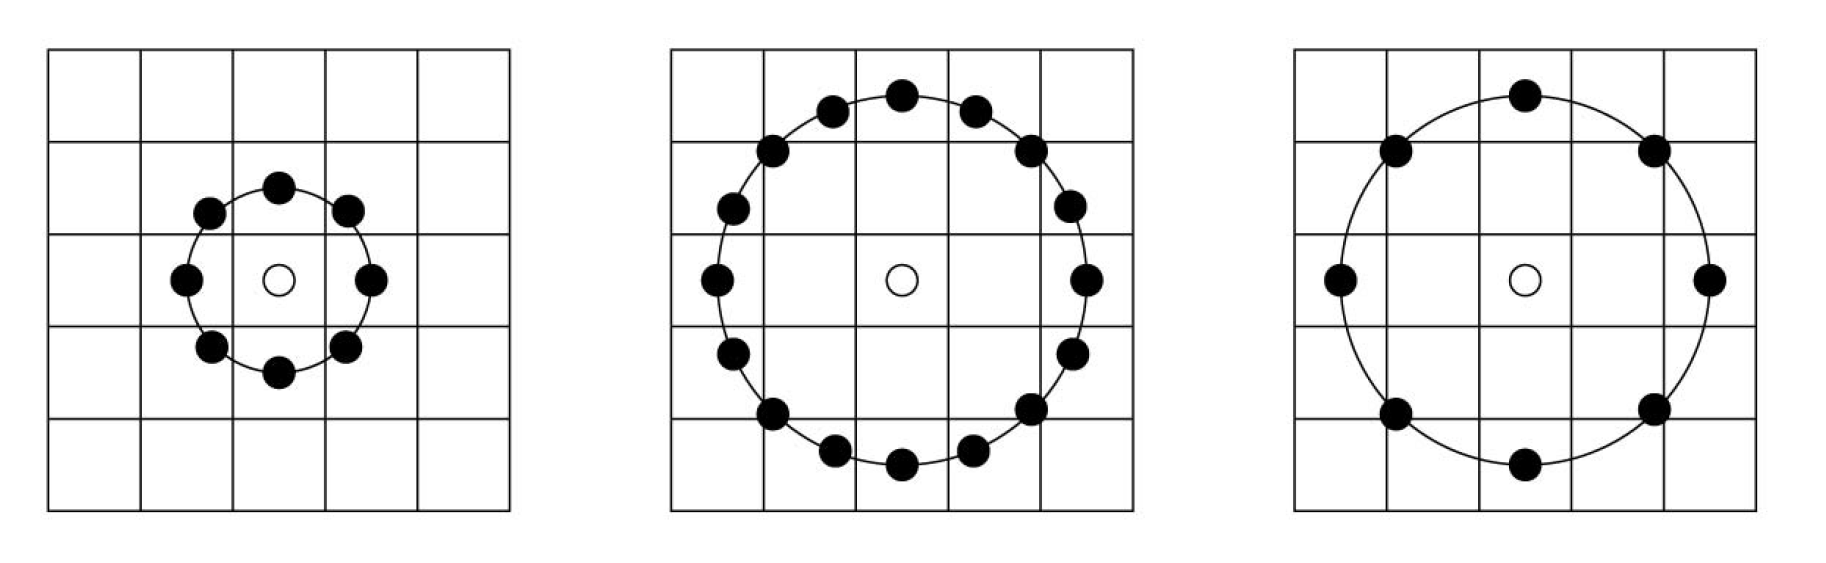
\includegraphics[width=253px]{./img/znazorneni_lbp.png}	
		\caption{Znázornění blocku Převzato z \cite{SrovnaniDeskriptoru}}
\end{figure}

\par Výpočet LBP probíhá podle následujícího vzorce, kde je pixel, pro který se hodnoty počítají, označen písmenem $c$ (centrální). Algoritmus následně prochází všechny okolní pixely označené písmenem  $x$. Hodnota daného pixelu je označena jako $p(x)$ a výsledek tohoto porovnání je označen $s(x)$.

\begin{displaymath} 
	\label{asd2} 
		    s(x) = \left\{ \begin{array}{r@{\quad}c}
    		1, & p(x) \geq h(c) \\
    		0, & p(x) < h(c) \\ \end{array} \right. 
\end{displaymath}

\begin{figure}[ht]
	\centering
	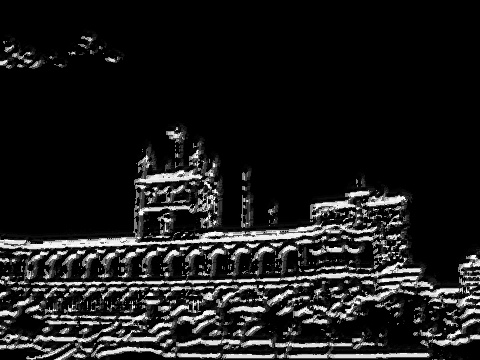
\includegraphics[width=150pt]{./img/lbp1_tau.jpg}
	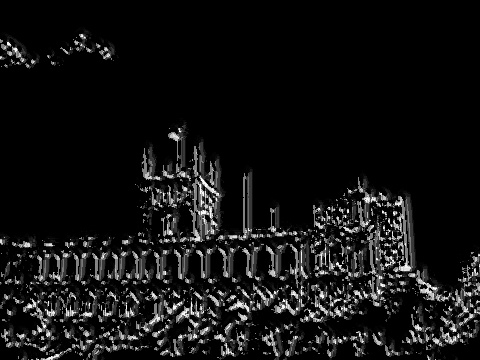
\includegraphics[width=150pt]{./img/lbp2_tau.jpg}
	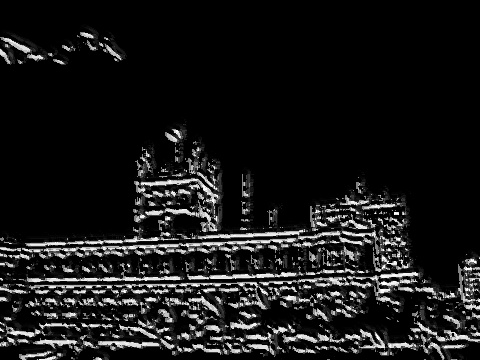
\includegraphics[width=150pt]{./img/lbp3_tau.jpg}
	\caption{Obrázky po aplikaci LBP s použitím $\tau$. Každý obrázek představuje jeden směr.}
\end{figure}

\subsection{Konstrukce globálního histogramu}
\par Obrázky získané z LBP jsou rozděleny pravidelnou čtvercovou mřížkou. Pro každou vzniklou oblast je vypočten lokální histogram. Vzniklé histogramy jsou zřetězeny. Díky tomu jsou získány tři histogramy, pro každý směr jeden, které jsou opět zřetězeny. \\
Rozdělení obrázků a určování lokálních histogramů se dělá za účelem zachování informace o prostorovém rozložení jednotlivých příznaků.

\section{Barevný POEM}
\subsubsection{Výpočet gradientu a magnitudy}
Výpočet gradientu probíhá obdobně jako u šedotónového obrázku. Pro každou ze tří složek jsou získány dvě matice filtrované maskami. Celkem bude $3 \times 2$ matic. Na matice se dá pohlížet jako na 2 vektory o 3 složkách. Vektory jsou sloučeny pomocí součtu vektorů do jednoho 3 složkového vektoru. Magnituda je opět velikost vektoru tentokrát ale v prostoru. \\
\\
Formát vzniklých vektorů 
\begin{align}
	\label{barevny_poem_vznikle_vektory}
			 u = [blue_x, green_x, red_x] \\
			 v = [blue_y, green_y, red_y]
\end{align}

Pomocí součtu vektorů je získán jeden třísložkový vektor:
\begin{align}
   \label{soucet_vektrou} \vec{u} + \vec{v} = (u_1 + v_1, u_2 + v_2, u_3 + v_3 )
\end{align} 

\begin{figure}[H]
    \centering
    \def\svgwidth{\columnwidth}
    \import{img/}{soucet_vektoru.pdf_tex} 
    \caption{Grafické znázornění součtu vektorů. Součet je tvořen z vektorů [4, 8, 10] a [8, 4, 0].}
    %\input{soucet_vektoru.pdf_tex}
\end{figure}

\subsubsection{Diskretizace směru gradientu}
U vektorů získaných v předchozím kroku je určena velikost úhlu mezi vektorem a ekvivalentním vektorem s vynulovanou složkou $z$. Následně je spočítáno do které části kružnice vektor směřuje. Pro znaménkovou reprezentaci je celkový rozsah $0 - \pi$, pro neznaménkovou reprezentaci $0 - 2\pi$.
\\
Při neznaménkové reprezentaci a počtu směrů $d = 3$ jsou následující intervaly $\left(0 - \frac{\pi}{3}\right)$, $\left(\frac{\pi}{3} - \frac{2\pi}{3}\right)$ a  $\left(\frac{2\pi}{3} - \pi\right)$.
\\
Pro výpočet diskretizace směru při neznaménkové reprezentaci je $y$ složka rozdělena na kladnou a zápornou část. To hraje velkou roli, pokud je $y$ složka vektoru záporná. V tom případě je nutné nebrat úhel $\alpha$, ale jeho doplněk ($ 2\pi - \alpha$).

\begin{figure}[H]
    \centering
    \def\svgwidth{\columnwidth}
    \import{img/}{3D_kruznice.pdf_tex} 
    \caption{Grafické znázorněnní součtu vektorů. Součet je tvořen z vektorů [4, 8, 10] a [8 4, 0].}
    %\input{soucet_vektoru.pdf_tex}
\end{figure}

\subsubsection{Výpočet lokálního histogramu}
\par Zbývající postup je totožný s POEMem. U každého směru se vezmou jednotlivé pixely s jejich okolím a zprůměrují se jejich hodnoty. 

\subsubsection{Zakódování příznaků pomocí LBP}
\par LBP operátor se aplikuje na kruhové okolí s poloměrem L/2 označeném jako block. Pro zvýšení stability je k centrálními pixelu přičítána malá konstanta~$\tau$. 

\begin{figure}[H]
	\centering
	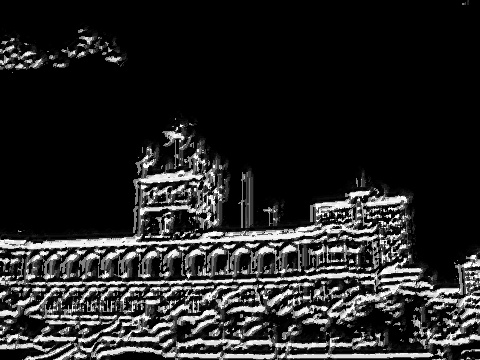
\includegraphics[width=150pt]{./img/lbp_3_1.jpg}
	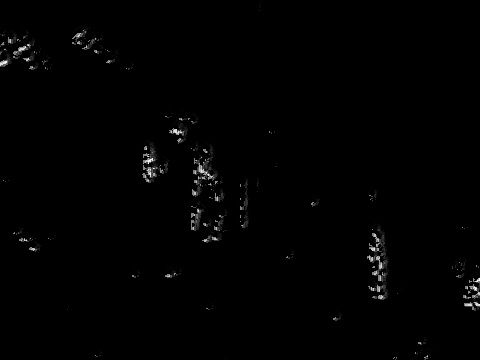
\includegraphics[width=150pt]{./img/lbp_3_2.jpg}
	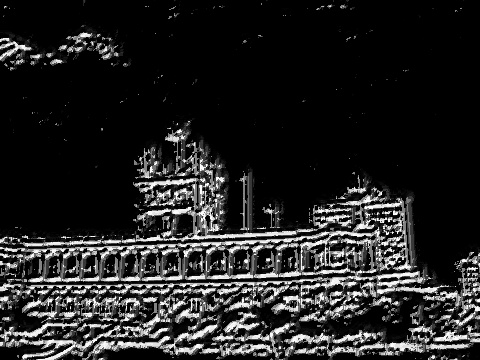
\includegraphics[width=150pt]{./img/lbp_3_3.jpg}
	\caption{Obrázky po aplikaci LBP s použitím $\tau$. Každý obrázek představuje jeden směr.}
\end{figure}

\subsubsection{Konstrukce globálního histogramu}
\par Obrázky získané z LBP jsou rozděleny pravidelnou čtvercovou mřížkou. Pro každou vzniklou oblast je vypočten lokální histogram. Vzniklé histogramy jsou zřetězeny přes všechny tři směry.

\chapter{Testovací databáze}
\par Pro natrénování a následné testování byla použita data z databází IAPRC a ESP. Obě databáze jsou standardně používané v automatické anotaci obrázků a jejich použítí umožní srovnání s literaturou. Kolekce obrázků na natrénování musí být pečlivě vybrána, aby zahrnovala co možná největši okruh z různých témat. 

\section{iaprtc12}
\par Sada iaprtc12 je kolekce obrázků přírodních scén, které zahrnují různé sporty a akce, fotografie lidí, zvířat, měst, krajin a mnoho jiných aspektů součastného života. Data obsahují \num{20 000} obrázků ve formátu \textit{jpg} s celkovým počtem \num{291} klíčových slov. Ke každému obrázku jsou přiložena metadata ve formátu \textit{XML}, která obsahují informace o obrázku v různých jazycích. Kromě angličtiny je tam i například španělština nebo němčina. V metadatatech ovšem nenajdeme klíčová slova tak, jak bychom si je představovali, ale v různých tagách nalezneme například titulek obrázku, který může vypadat jako The Plaza de Armas. V tagu description je například  a woman and a child are walking over the square. Spolu s databází byla získána i klíčová slova, která byla z přiložených xml extrahována.\\
K jednomu obrázku je v průměru přiřazeno \num{5.7} klíčových slov. Pro trénovaní bylo použito \num{17 664} obrázků, na následné testování jich bylo použito \num{1960} \cite{ESPvon2004labeling}. 


\begin{figure}[h]
		\centering
		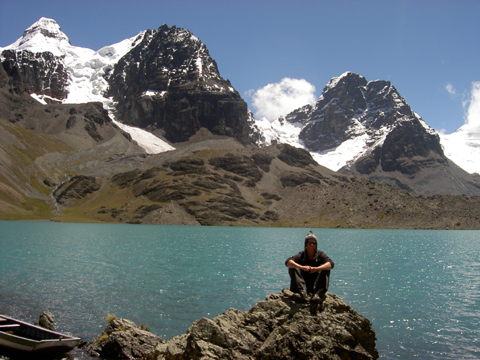
\includegraphics[width=140px]{./img/iaprtc12.jpg}	
		\caption{Ukázka obrázku s klíčovými slovy: front lake man mountain rock sky summit}
\end{figure}

\section{ESP}
\par Sada ESP obsahuje širokou škálu snímku s anotacemi, ze kterých byla použita jen malá část. Konkrétně \num{18 689} obrázků na trénování a \num{2061} na testování. Ke každému obrázku je přiřazen soubor ve formátu \textit{desc}, který obsahuje anglické anotace. Z celkových 269 klíčových slov je k jednomu obrázku přiřazeno v průměru 4.6 slov.

\par Obrázky získaly svá klíčová slova pomocí ESP game, což je hra, která funguje pouze online. V principu spojí dva hráče, kteří nemají možnost spolu komunikovat. Následně je oběma hráčům zobrazen stejný obrázek, který musí popsat co nejvíce různými výrazy v angličtině. V případě, že se hráči shodnou, počítač předpokládá, že mu poskytli pravdivou informaci o tom, co se na obrázků nachází. Tak si tuto anotaci uloží do databáze a hráči získají body.

\begin{figure}[h]
		\centering
		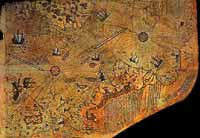
\includegraphics[width=140px]{./img/esp.jpg}	
		\caption{Ukázka obrázku s klíčovými slovy: brown chart country map old orange ship white}
\end{figure}

%Výhodou této sady je, že řeší problém kolektivnýho významu mezi anotátory což vede k anotaci s méně individuální předpojatostí.
%Výhodou této sady je že lidská anotace odráží kolektivní sémantiku dohodu mezi anotátory což vede k anotaci s méně individuální %předpojatostí


\chapter{Evaluační metriky}
\par Kvalitu a úspěšnost klasifikátoru udává přesnost (precision) a úplnost (recall). Přesnost udává jak moc jsou výsledky relevantní a úplnost kolik skutečně relevantních výsledků bylo přiřazeno. V případě, že přesnost převyšuje úplnost, jsou klíčová slova sice korektní, ale je jich málo. V opačném případě při převyšující úplnosti bylo získáno hodně klíčových slov, ale málo z nich je korektních. Proto je snaha získat obě čísla co nejvyšší. Níže jsou uvedeny dva postupy pro výpočet přesnosti a úplnosti \cite{Result_A_A}.  V práci je použitý postup per word, stejně jako je uvedeno v článku \citep{JEC}. 
\par Počet nenulových slov značí počet slov, která byla při anotaci použita alespoň jednou. 

\section{Přesnost a úplnost pro celý klasifikátor}
\par \textit{TP} (True Positive) značí klíčová slova, která měla být k obrázku klasifikátorem přiřazena a skutečně mu přiřazena byla. \textit{FP} (False Positive) určuje klíčová slova, která k danému obrázku nepatří, avšak klasifikátor je přiřadil. \textit{FN} označuje klíčová slova, která k obrázku patří a klasifikátor je nepřiřadil. 

\begin{multicols}{2}
	\begin{figure}[H]
		    \centering
    	%\def\svgwidth{\columnwidth}
    	%\import{img/}{recall_precision.pdf_tex} 
		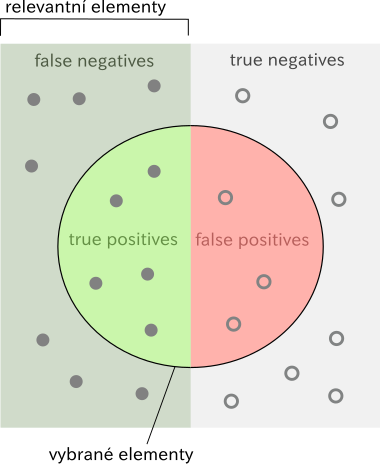
\includegraphics[height=180px]{./img/recall_precision.png}
		\caption{Znázornění precision a recall.}
	\end{figure}
	\begin{center}
		\begin{align}
   			\label{precision2} Prec &= \frac{TP}{TP + FP} \\[30pt]
   			\label{recall2} Rec &= \frac{TP}{TP + FN}
		\end{align}

	\end{center}
\end{multicols}

\section{Přesnost a úplnost - per word}
\par Zpracování precision a recall probíhá pro každé slovo v testovací sadě (proto také per word). Výpočet probíhá jako porovnání anotací přidělených člověkem s anotacemi přidělenými klasifikátorem. $w_{auto}$ představuje počet obrázků, kterým bylo dané slovo přiřazeno klasifikátorem, $w_{human}$ počet obrázků, kterým bylo dané slovo přiřazeno člověkem a $w_{corrrectly}$ počet obrázků, kterým bylo slovo přiřazené správně. 

\par Recall \eqref{recall} je počet obrázků správně anotovaných s daným slovem děleno počtem obrázků, kterým bylo toto slovo přiděleno v anotaci člověkem. Precision \eqref{precision} je počet správně anotovaných obrázků s tímto slovem děleno celkovým počtem anotovaných obrázků s tímto slovem (správně nebo ne). 

\begin{align}
   \label{recall} Rec = \frac{w_c}{w_h}
\end{align}
\begin{align}
   \label{precision} Prec = \frac{w_c}{w_a}
\end{align}

\par Výsledná precision a recall se počítá jako průměr dosažených výsledků pro jednotlivá slova. 

\section{F-measure}
F-measure je měřítkem úspěšnosti klasifikace a je definována jako harmonický průměr precision a recall. \eqref{f-measure} Jak již bylo výše zmíněno, klasifikátor dosahuje nejlepších výsledků právě tehdy, když precision a recall dosahují co nejvyších hodnot, avšak zároveň jsou vybalancovány. Pokud tedy bude klasifikátor optimalizován pouze pro jednu z těchto hodnot, a tím znevýhodněna druhá, harmonický průměr se rychle sniží. V literatuře na anotaci obrázku se však F-measure běžně neobjevuje.

\begin{align}
   \label{f-measure} F-measure = 2 \cdot \frac{precision \cdot recall}{precision + recall}
\end{align}


\chapter{Návrh systému}
Systém byl navržen jako modulární z důvodu snadné obměny některé z častí. Problém automatické anotace obrázků se dá rozdělit do několika částí. Extrahování příznaků z dat, samotná klasifikace a v neposlední řadě vyhodnocení úspěšností klasifikace. Pro efektivnější použití bylo navrženo i ukládání mezivýsledků. Návrh systému je zobrazen na následujícím obrázku.


\begin{figure}[ht]
    \centering
    \label{navrh_systemu}
    \def\svgwidth{\columnwidth}
    \import{img/}{navrh_systemu.pdf_tex} 
    \caption{Návrh systému.}
    %\input{soucet_vektoru.pdf_tex}
\end{figure}


\chapter{Implementace}
\section{Použité programové prostředky}
\par Program byl navržen na operační systém Linux. Jako programovací jazyk byl zvolen Python, a to z důvodu jeho jednoduchého použití. To je pro tento prototyp velice výhodné na časovou náročnost a zároveň je pro Python k dispozi hodně knihoven. 

\par Pro spuštění programu je třeba mít nainstalovaný Python ve verzi 2.7.12 s NumPy verze 9, knihovnu openCV verzi 3.1 a vědeckou knihovnu scipy verze 0.17.0. Vzhledem k náročnosti programu je pro jeho spuštění nutné mít v počítači alespoň 16 GB RAM paměti a to především z důvodů ukládání mezivýsledků pomocí modulu \textit{pickle}, což je modul pro serializaci objektů. Následující postupy jsou uvedeny pro operační systém Linux, a tak se mohou od postupu na jiném operačním systému lišit.   
  
  
\subsection{OpenCV}
\par OpenCV (Open source computer vision) je knihovna vydávána pod licencí BSD a je volně k dispozici jak pro akademické účely, tak pro komerční použití. Je vhodná pro použití v C++, C, Python a Javě. Podporuje operační systémy Windows, Linux, Mac OS, iOS a Android.

\par Knihovna byla navrhnuta pro výpočetní efektivitu v oblasti počítačového vidění a zpracování obrazu se zaměřením na zpracování obrazu v reálném čase. Z důvodu optimalizace byla napsána v C/C++. 

\par Knihovna OpenCV je dostupná na adrese: http://opencv.org/

\subsection{Scikit}
\par Scikit-image je vědecká knihovna algoritmů pro zpracování obrazu. Je k dispozici zdarma a bez omezení s licencí BSD. Poskytuje dobře zdokumentované API v programovacím jazyce Python a je vyvíjena aktivním mezinárodním týmem spolupracovníků.
\cite{Scikit}

\section{Modulové jednotky programu}
Pro snadné spuštění programu je pro uživatele připraven skript \textit{run.py}, který postupně spouští jednotlivé moduly. Moduly je možné spouštět i odděleně.
\subsection{Config}
\par Při spuštění programu je nejdříve načten konfigurační soubor, který obsahuje jeho veškerá nastavení. Mimo jiné zde najdeme cesty k souborům, ze kterých program načítá data nebo cesty k soubourům, do kterých data naopak ukládá. Dále jsou v cofingu uvedené jednotlivé metody s očekávanou hodnotou \textit{True} nebo \textit{False} v závislosti zda se mají použít nebo ne a nastavení vzdáleností, které se mají na jednotlivé příznaky použít.

\subsection{Load data}
\par Modul pomocí funkce \textit{load\_pictures} načte obrázky z listů uvedených v configu (\textit{TRAIN\_LIST} a \textit{TEST\_LIST}). Následně je na všechny obrázky zavolána funkce \textit{load\_features}, která načte příslušné příznaky. Nakonec jsou celé stuktury listů testovacích nebo trenovacích obrázku uloženy do souboru, dle configu \textit{DATAFILE\_TRAIN} popřípadě \textit{DATAFILE\_TEST}.


\subsubsection{Extrakce příznaků}
%\label{sec:extrakce_priznaku}
\par Jednotlivé výpočty příznaků jsou rozděleneny do zvláštních modulů, aby byla obměna jejich výpočtu snadno nahraditelná. V každém modulu je stěžejní pouze funkce \textit{count\_} a název příslušné metody (např. \textit{count\_haarq}), která je volána právě z modulu load data.

\par Při počítání barevných histogramů byl zjištěn překvapivý poznatek. V~případě, kdy je histogram jako datová struktura \textit{list} a až výsledný histogram převeden do \textit{numpy array}, je rychlost programu nesrovnatelně větší oproti tomu, když jsou histogramy vytvořeny rovnou jako \textit{numpy array}.  

\par Za zmíňku také stojí převádění výsledných matic na vektor, kdy v případě převádění vektoru do 16 prvkové podoby, výsledné číslo může dosahovat i nejvyšší hodnoty. V této situaci je výsledné číslo posunuto na poslední index vektoru. Toto řešení se mimo jiné zobrazuje v případě příznaku HaarQ. 

\par V případě získávání příznaku z POEMu a barevného POEMU byl obrázek před výpočtem zmenšen na polovinu z důvodu rychlejšího průběhu.

\par U většiny příznaků byla použita knihovna OpenCV. U Gabora byla použita knihovna scikit, která si ksize určuje podle parametrů vlny tzn. tento parametr nezadáváme.
   
  
\subsection{Knn classifier}
\par V tomto modulu probíhá počítání vzdáleností mezi jednotlivými příznaky (vektory). Ve funkci \textit{count\_all\_distance} je v jednom běhu cyklu zjištěna jak vzdálenost mezi příznaky testovaného obrázku se všemi obrázky z trénovací sady, tak i určeno jejich maximum a minimum. Dále je volána metoda \textit{count\_jec}, která vzdálenosti za pomocí zjištěného maxima a minima přeškáluje na interval 0 až 1. Naškálovanou hodnotu přičte do celkové sumy vzdáleností. V konečné fázi je suma vzdáleností podělena počtem příznaků. Vznikne tak výsledná vzdálenost JEC.
    

\subsection{Label transfer}
\par Modul pro přenost klíčových slov má dvě modifikace. Mezi modifikacemi je možno přepínat pomocí parametru \textit{LABEL\_TRANSFER} v configu. 

\par Při variantě, kdy je přenesení provedeno pomocí originálního algoritmu pro přenesení klíčových slov, jsou předpočteny četnosti klíčových slov v trénovacích datech pomocí funkce \textit{count\_keyword\_frequency\_train\_set}, následováno předpočtením frekvence výskytu klíčových slov s ostaními klíčovými slovy ve funkci \textit{frequency\_word\_with\_other\_word\_dictionary}. Pro každý obrázek následuje funkce \textit{label\_transfer}. V této funkci se již přiřazují samotná klíčová slova od prvního souseda. Pokud je zjištěno, že od prvního souseda je dostatek klíčových slov, je funkce je ukončena. V opačném případě pokračuje do funkce \textit{add\_keywords\_from\_neighbors}, která dodá potřebná klíčová slova od dalších k nejbližších sousedů. Nakonec jsou klíčová slova uložena do souboru dle configu.

\par Druhou variantou je dynamické přenesení klíčových slov pomocí prahování. Zde je rovnou spuštěna funkce \textit{label\_transfer} pro každý obrázek a jsou přenesena klíčová slova přesahující hodnotu práhu. V konečné fázi jsou klíčová slova uložena do souboru dle configu. 

\par Při přenášení klíčových slov pomocí prahování na databázi ESP při pěti nejbližších sousedech byl objeven problém při počítání prahu. V případě, kdy má $K$ nejbližších sousedů pouze jedno totožné klíčové slovo, ve vzorečku pro práh by jmenovatel vyšel nula. Proto je doplněna podmínka a v této situaci je jediné klíčové slovo přeneseno i bez výpočtu prahu. 
  

\subsection{Evaluator}
\par Tento modul vyhodnotí úspěšnosti anotace. Jako první získáme všechna klíčová slova a to pomocí funkce \textit{getKeywords}. Pokračujeme získáním anotovaných dat ve funkci \textit{read\_data\_from\_file}.  Následně je pro každé klíčové slovo spočítána přesnost a úplnost. Tyto hodnoty jsou popsány v sekci Vyhodnocení výsledků.

\section{Doby běhu programu}
\par Doby běhu programu jsou v řádu hodin. S nejdelším časem je možné se setkat u modulu Load data. Jeho doba běhu závisí na načítaných příznacích a může přesahovat i 12 hodin. Za zmíňku stojí i modul \textit{Knn classifier}, který následuje \textit{label transfer} a jejich doba běhu se může pohybovat kolem 1 hodiny. Jak již bylo výše zmíněno, doba běhu se dá ovlivnit použitými konstrukcemi. Například rozdíl použití \textit{listu} a \textit{numpy array}.
Pokud by se tento prototyp překlápěl do efektivnějšího programovacího jazyku jako je například C, byla by doba běhu optimálnější. V tomto případě byla důležitější rychlost vývoje.

\chapter{Vyhodnocení výsledků}

\section{Srovnání výsledků}
Přesné parametry se kterými autoři článku \cite{JEC2} dosahovali nejlepších výsledků, nebyly zjištěny, proto bylo třeba je u některých příznaků zkoušet metodou pokus omyl. 


\subsection{Gabor - porovnání parametrů}
Gabor patří mezi příznaky u kterých nebyl uveden přesný postup zpracování příznaků. Byly pouze zmíněny tři vlnové délky a čtyři orientace. Z tabulky \ref{tabulka:gabor} je zřejmé, že algoritmus dosahoval nejlepších výsledků při použití filtrů s vlnovými délkami $0.25$, $0.5$, $1.0$ a orientacemi $0$, $\frac{\pi}{4}$, $\frac{\pi}{2}$, $\frac{3}{4}\pi$. Tyto nejúspěšnější parametry byly také použity v metodě JEC.
\begin{center}
\begin{tabular}{ |c|c|c|c|c| }
\hline
Parametry & $P_{\%}$ & $R_{\%}$ & N \\ \hline
 lambda $0.25$, $0.5$, $1.0$ & \multirow{3}{*}{9.9} & \multirow{3}{*}{6.8} & \multirow{3}{*}{151} \\
 sigma $1$ & & & \\
 theta $0$, $\frac{\pi}{4}$, $\frac{\pi}{2}$, $\frac{3}{4}\pi$ & & & \\ \hline
 lambda 2, $2\sqrt{2}$, 4 & \multirow{3}{*}{8.5} & \multirow{3}{*}{5.7} & \multirow{3}{*}{143} \\
 sigma $1$ & & & \\
 theta $0$, $\frac{\pi}{4}$, $\frac{\pi}{2}$, $\frac{3}{4}\pi$ & & & \\ 
\hline
\end{tabular}
\captionof{table}{Gabor s knihovnou scikit na datech iaprtc12.}
\label{tabulka:gabor}
\end{center}

\subsection{Haar - porovnání parametrů}
U Haara byly vyzkoušeny dvě možnosti vytváření deskriptoru. Deskriptor jako vektor 12x16 prvků je označena metoda, kdy byla výsledná matice z každé velikosti i orientace převedena na 16ti prvkový vektor. 
\par Dalsí možností je udělat skrz výslednou matici její průměr. Výsledným vektorem bude v tomto případě 12ti prvkový vektor průměrů. Z následující tabulky je vidět, že jednodušší vektor průměrů je úspěšnější, proto také bude použit u metody JEC.
\newpage
\begin{center}
	\begin{tabular}{ |c|c|c|c| }
		\hline
		Parametry & $P_{\%}$  & $R_{\%}$ & N \\ \hline
		Desktiptor jako vektor $12 \times 16$ prvků & 2.9 & 2.1 & 63 \\ \hline
		Deskriptor jako vektor průměrů & 5.8 & 4 & 114 \\ \hline 	
	\end{tabular}
	\captionof{table}{Haar na datech iaprtc12.}
\end{center}

\subsection{Přiřazování klíčových slov pomocí prahování}
Při testování metody přiřazování klíčových slov pomocí prahování bylo vyzkoušeno nastavení klasifikátoru na 5, 8 a 10 sousedů. Při nahlédnutí do následujících tabulek je možné si povšimnout, že vyhodnocení klasfikace vyšlo nejlépe pro 8 sousedů.  
\begin{center}
\begin{tabular}{l | c c c| c c c|c c c}
		          	& \multicolumn{3}{c|}{5 sousedů} & \multicolumn{3}{ c}{8 sousedů} & \multicolumn{3}{ c}{10 sousedů} \\ 
Metoda          		& $P_{\%}$ & $R_{\%}$ & N & $P_{\%}$ & $R_{\%}$ & N & $P_{\%}$ & $R_{\%}$ & N \\
\hline
RGB						& 20.1 & 9 & 178 & 15.7 & 12.9 & 195 & 14.3 & 15.3 & 205 \\
LAB					  	& 17.1 & 8.8 & 156 & 14.3 & 12.4 & 172 & 14.4 & 14.7 & 185 \\
HSV            			& 21 & 11.4 & 191 & 17.2 & 16.4 & 213 & 14.9 & 18.6 & 221 \\
RGB, LAB, HSV      		& 21.9 & 11.2 & 188 & 18.8 & 16.9 & 218 & 16.1 & 19 & 221 \\
Gabor					& 12 & 5.9 & 137 & 9.1 & 8.6 & 154 & 8 & 10.4 & 165  \\  
GaborQ					& 3.9 & 2.4 & 81 & 4.6 & 5.1 & 115 & 4.2 & 6.5 & 124 \\
Haar					& 4.9 & 2.6 & 85 & 4.3 & 4.4 & 108 & 3.8 & 5.5 & 118 \\  
HaarQ					& 8 & 3.2 & 102 & 5.8 & 5.3 & 122 & 5 & 6.6 & 130 \\ 
\hline
\hline
JEC						& 23.8 & 12.3 & 189 & 19.7 & 17.7 & 212 & 17.1 & 19.9 & 215 \\ 
POEM					& 27.2 & 14.3 & 200 & 22.7 & 20.1 & 223 & 20 & 23 & 230 \\
RGB, LAB, HSV, POEM		& 26.3 & 15 & 206 & 22.1 & 20.9 & 234 & 19.5 & 23.3 & 238 \\
Barevný POEM			& 22.8 & 13.4 & 187 & 20 & 18.1 & 209 & 18.1 & 20.9 & 214 \\
\end{tabular}
\captionof{table}{Výsledky získané přiřazováním klíčových slov s prahem na datech iaprtc12. P značí přesnost, R úplnost a N počet nenulových klíčových slov.}
\end{center}

\begin{center}
\begin{tabular}{l | c c c| c c c|c c c}
		          	& \multicolumn{3}{c|}{5 sousedů} & \multicolumn{3}{ c}{8 sousedů} & \multicolumn{3}{ c}{10 sousedů} \\ 
Metoda          		& $P_{\%}$ & $R_{\%}$ & N & $P_{\%}$ & $R_{\%}$ & N & $P_{\%}$ & $R_{\%}$ & N \\
\hline
RGB						& 17.6 & 8.9 & 170 & 13.1 & 12.6 & 195 & 11.1 & 14.4 & 202 \\
LAB					  	& 7.9 & 4.1 & 95 & 7.7 & 6.5 & 121 & 7.4 & 8.2 & 133 \\
HSV            			& 19 & 11 & 192 & 14 & 14.8 & 205 & 11.9 & 16.4 & 207 \\
RGB, LAB, HSV      		& 20.4 & 11 & 182 & 14.4 & 14.8 & 201 & 12.1 & 16.9 & 206 \\
Gabor 					& 14.8 & 7.5 & 153 & 10.5 & 10.3 & 170 & 8.9 & 11.9 & 179 \\
GaborQ					& 13.6 & 6.1 & 145 & 9 & 8.4 & 164 & 7.6 & 10 & 171 \\
Haar					& 10.1 & 4.5 & 121 & 6.9 & 6.4 & 141 & 5.7 & 7.6 & 149 \\
HaarQ					& 8.9 & 3.3 & 103 & 7.1 & 5.3 & 125 & 5.9 & 6.5 & 134 \\				
\hline
\hline
JEC						& 21.6 & 11.6 & 195 & 15.3 & 15.3 & 206 & 13.1 & 17.2 & 210 \\ 
POEM                   & 21.6 & 7.7 & 159 & 16 & 10.7 & 175 & 13.7 & 12.4 & 180 \\
RGB, LAB, HSV, POEM		& 22.4 & 12.1 & 193 & 16.7 & 16.3 & 212 & 14.3 & 18.3 & 213 \\
Barvený POEM			& 18. 5 & 8.6 & 167 & 14 & 11.7 & 182 & 11.9 & 13.2 & 186 \\
\end{tabular}
\captionof{table}{Výsledky získané přiřazováním klíčových slov s práhem na datech esp. P značí přesnost, R úplnost a N počet nenulových klíčových slov.}
\end{center}

\subsection{Konečné výsledky a srovnání s literaturou}
\par Při konečném srovnání výsledků z článku \cite{JEC2} je možné si povšimnout, že ačkoliv u barevných příznaků byl postup vytvoření histogramu přesně určen, nebylo dosaženo stejně úspěšných výsledků. Je ovšem možné, že autoři obrázky před klasifikací předzpracovávali (změna velikostí obrázků atd.). Následuje výpis parametrů, díky kterým byly výsledky získány.\\
\vspace{0.5cm}

\setlist{nosep}
\begin{description}
	\item[klasifikátor] \hfill 
		\begin{itemize}	
			\item Počet sousedů: 5
			\item Počet klíčových slov: 5
			\item Přenášení klíčových slov pomocí originálního algoritmu uvedeného u metody JEC
		\end{itemize}
	\item[RGB, HSV] \hfill 
		\begin{itemize} 
			\item $3\times 16$ binový histogram
			\item Vzdálenost: L1 	
		\end{itemize}
	\item[LAB] \hfill 
		\begin{itemize} 
			\item $3\times 16$ binový histogram
			\item Vzdálenost: KL 	
		\end{itemize}		
	\item[Gabor, GaborQ] \hfill 
		\begin{itemize} 
			\item $12 \times 16$ prvkový vektor
			\item Vzdálenost: L1 
			\item Lambda: $0.25$, $0.5$, $1.0$ 
			\item Sigma: $1$
			\item Theta: $0$, $\frac{\pi}{4}$, $\frac{\pi}{2}$, $\frac{3}{4}\pi$  	
		\end{itemize}
	\item[Haar, HaarQ] \hfill 
		\begin{itemize} 
			\item $12$ prvkový vektor
			\item Vzdálenost: L1 
			\item Filtry: [1.0, 1.0], [-1.0,-1.0]; [-1.0, 1.0], [-1.0, 1.0]; [1.0, -1.0], [-1.0, 1.0]  	
		\end{itemize}
	\item[POEM] \hfill 
		\begin{itemize} 		
			\item Vzdálenost: L1
			\item Počet směrů: 3
			\item Velikost cellu: 3
			\item Velikost blocku: 8
			\item Tau: 4 	
		\end{itemize}
	\item[Barevný POEM] \hfill 
		\begin{itemize} 
			\item Vzdálenost: L1 
			\item Počet směrů: 3
			\item Velikost cellu: 3
			\item Velikost blocku: 8
			\item Tau: 4  	
		\end{itemize}
\end{description}


\vspace{0.5cm}

\newpage
\begin{center}
\begin{tabular}{l | c c c|c c c}
		          	& \multicolumn{3}{c|}{IAPRTC12} & \multicolumn{3}{ c}{ESP} \\ 
Metoda          		& $P_{\%}$ & $R_{\%}$ & N & $P_{\%}$ & $R_{\%}$ & N \\
\hline
RGB						& 14.1 & 9 & 167 & 17 & 13.2 & 209 \\
LAB					  	& 12.7 & 7.5 & 148 & 6.1 & 5.2 & 117 \\
HSV            			& 16.7 & 10.9 & 181 & 18.2 & 14.8 & 211 \\
RGB, LAB, HSV      		& 17.4 & 11.1 & 178 & 18.7 & 14.8 & 209 \\
Gabor					& 8.1 & 4.7 & 126 & 14.4 & 11.4 & 194 \\
GaborQ					& 6.9 & 4.8 & 133 & 11.6 & 9.1 & 187 \\
Haar					& 5.8 & 4 & 114 & 10.2 & 8.4 & 178 \\
HaarQ					& 5.8 & 4.4 & 123 & 9.4 & 7.3 & 169 \\
\hline
\hline
JEC						& 17.3 & 11.6 & 182 & 19.6 & 14.8 & 210 \\ 
POEM		     		& 21.5 & 12.8 & 189 & 18.1 & 12.1 & 195 \\
RGB, LAB, HSV, POEM		& 21.8 & 13.8 & 187 & 20 & 15.6 & 201  \\
Barevný POEM			& 21 & 12.4 & 184 & 17.4 & 13 & 200 \\
\end{tabular}
\captionof{table}{Výsledky získané v rámci práce. P značí přesnost, R úplnost a N počet nenulových klíčových slov. V případě kombinace RGB, LAB, HSV a POEMu byl použit originální algoritmus pro přenost klíčových slov uvedený u metody JEC.}
\end{center}

\begin{center}
	\begin{tabular}{l | c c c|c c c}
		          	& \multicolumn{3}{ c|}{IAPRTC12} & \multicolumn{3}{ c }{ESP} \\ 
	Metoda          		& $P_{\%}$ & $R_{\%}$ & N & $P_{\%}$ & $R_{\%}$ & N  \\
	\hline
	RGB						& 20 & 13 & 189 & 21 & 17 & 221 \\
	LAB					  	& 22 & 14 & 194 & 20 & 17 & 221 \\
	HSV            			& 18 & 12 & 190 & 18 & 15 & 217  \\
	Haar					& 17 & 8 & 161 & 21 & 14 & 210  \\
	HaarQ					& 16 & 10 & 173 & 19 & 14 & 210 \\
	Gabor					& 14 & 9 & 169 & 16 & 12 & 199 \\
	GaborQ					& 8 & 6 & 137 & 14 & 11 & 205 \\
	\hline
	\hline
	JEC						& 25 & 16 & 196 & 23 & 19 & 227 \\ 
	\end{tabular}
	\captionof{table}{Výsledky z literatury \cite{JEC2}.}
\end{center}


\begin{figure}[H]
	\centering
	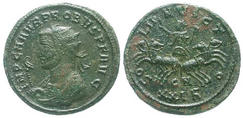
\includegraphics[width=140px]{./img/esp_86743.jpg}	
	\caption{Ukázka obrázku ze sady ESP.}
	\label{img:esp_coin}
\end{figure}

\begin{center}
	\begin{tabular}{| p{7cm} | p{7cm} |}
		\hline
		\textbf{Získání klíčových slov} & \textbf{Klíčová slova} \\ \hline
		Originální klíčová slova & circle coin face head metal money old round silver \\ \hline
		JEC s deskriptory RGB, HSV, LAB, Gabor, GaborQ, Haar a HaarQ & man old metal coin money \\ \hline
		JEC s deskriptory POEM, RGB, HSV a LAB & man old metal coin money  \\ \hline 
		POEM rozšířenou na všechny barevné kanály & face old head coin money \\ \hline 
		JEC s deskriptory RGB, HSV, LAB, Gabor, GaborQ, Haar a HaarQ s přenášením klíčových slov pomocí prahování & old money coin \\ \hline 
		JEC s deskriptory POEM, RGB, HSV a LAB s přenášením klíčových slov pomocí prahování & old money coin \\ \hline
		POEM rozšířenou na všechny barevné kanály s přenášením klíčových slov pomocí prahování & old money coin\\ \hline 
			
	\end{tabular}
	\captionof{table}{Klíčová slova k obrázku \ref{img:esp_coin}}
\end{center}
	 

\chapter{Závěr}
\par V práci byla řešena automatická anotace obrázků pomocí spojování barevných a texturových příznaků. U prvního řešení s metodou JEC probíhalo vyhodnocení a klasifikace příznaků odděleně a poté byla výsledná klasifikace spojena z několika částí. V druhém případě bylo spojení příznaků interpretováno jako jeden společný příznak, kdy byl POEM rozšířen na všechny barevné kanály.
\par V teoretické části byly popsány a rozebrány nízkoúrovňové příznaky barva a textura. U barvy se zabývalo barevnými modely RGB, LAB a HSV. U textury to byl Gabor, Haar a POEM. Dále byla pozornost kladena na přenášení klíčových slov za pomocí práhu, kdy musela frekvence výskytu u sousedů převýšit stanovený práh. 
\par V realizační části byl navržen a implementován program v jazyce Python pro automatickou anotaci obrázků, který využívá právě vyše zmíněné barevné prostory a reprezentace textur. Na základě naměřených výsledků byly laděny optimální parametry. V rámci práce byla prostudovaná a použita knihovna openCV. Funkčnost programu byla otestována na databázích iaprtc12 a ESP.
\par Po vyhodnocení dosažených výsledků a porovnání s literaturou bylo zjištěno, že nebylo dosaženo tak vysokých hodnot přenosti a úplnosti klasifikátoru jako uvádějí autoři článku \citep{JEC2}. V některých případech se dá předpokládat, že to může být z důvodu neznalosti přesných parametrů, avšak u barevných příznaku (RGB, HSV a LAB), kdy byly uvedeny přesné parametry a postup sestavení příznaků je nesouhlasnost výsledků vysoce zvláštní. 
\par Do budoucna jako vylepšení se nabízí úprava barevného POEMu, kdy by se diskretizace směru gradientu nezaměřovala ve třírozměrném prostoru pouze na 3 směry v rovině, ale brala by v potaz celé postavení vektoru v rovině, tím pádem by vznikla kupole o 9 částech (směrech). Ohledně metody JEC by vylepšením bylo použít další deskriptory. 

% 
% PRO ANGLICKOU SAZBU JE NUTNÉ ZMĚNIT
% CITAČNÍ STYL!
%

\chapter{Použité zkratky}


\begin{labeling}{zkratky}
	\item [AIA] Automatic image anotation.	
	\item [JEC] Joint equal contribution
	\item [RGB] Barevný model Red, Green, Blue (červená, zelená, modrá).
	\item [LAB] Barevný model. 
	\item [HSV] Barevný model. 
	\item [POEM] Patterns of oriented edge magnitudes.
	\item [LBP] Local binary pattern.
	\item [OpenCV] Open source computer vision.
	\item [BSD] Licence pro svobodný software, umožňující volné šíření softwaru.
	\item [KL - divergence] Kullaback-Leibler divergence.
\end{labeling}

\nocite{*}
\bibliographystyle{csplainnatkiv}
{\raggedright\small
\bibliography{literatura}
}

\appendix
\chapter{Uživatelská dokumentace}
\par Pro spuštění programu je třeba mít nainstalovaný python ve verzi 2.7.12 s NumPy verze 9, knihovnu openCV verzi 3.1 a vědeckou knihovnu scipy verze 0.17.0. Vzhledem k náročnosti programu je pro jeho spuštění nutné mít v počítači alespoň 16 GB RAM paměti. Následující postupy jsou uvedeny pro operační systém Linux. Na jiném operačním systému se mohou postupy lišit.

\par Veškeré nastavení aplikace probíhá pomocí souboru \textit{config.py}

\vspace{1cm} 
\noindent Parametry configu:
\begin{itemize}
	\item \textit{TRAIN\_LIST} - Trénovací list obrázků, který by měl obsahovat cesty k obrázkům trénovací sady a jejich klíčová slova ve formátu \textit{cesta\_k\_obrazku; klíčové\_slovo další\_klíčové\_slovo}. Předpokládaný formát je \textit{.txt}.
	\item \textit{TEST\_LIST} - Testovací list, který by měl obsahovat cesty k obrázkům testovací sady a jejich klíčová slova ve formátu \textit{cesta\_k\_obrázku; klíčové\_slovo klíčové\_slovo}. Předpokládaný formát je \textit{.txt}.
	\item \textit{DATAFILE\_TRAIN} - Soubor, do kterého budou uloženy příznakové vektory načtených obrázků z trénovací sady. Předpokládaný formát \textit{.pyc}.
		\item \textit{DATAFILE\_TEST} - Soubor do kterého budou uloženy příznakové vektory z načtených obrázků z testovací sady. Předpokládaný formát \textit{.pyc}.
	\item \textit{PICTURE\_RESULT} - Obsahuje názvy obrázků a klíčová slova přiřazena klasifikátorem.
	\item \textit{PICTURE\_ALL\_KEYWORDS} - Obsahuje názvy obrázků s přiřazenými slovy od klasifikatoru i s se slovy přiřazené člověkem. Ve formátu \textit{cesta\_k\_obrázku;originální\_klíčová\_slova;klíčová\_slova\_přiřazena\_klasifikátorem}
	\item \textit{KEYWORDS\_RESULT} - Cesta k souboru, který obsahuje výsledky klíčových slov, jejich přesnost a úplnost.
	\item \textit{COUNT\_NEIGHBORS} - Počet sousedů.
	\item \textit{COUNT\_KEYWORDS} - Počet klíčových slov.
	\item \textit{LABEL\_TRANSFER} - Určuje způsob přiřazování klíčových slov. Při hodnotě \textit{TH} bude použíté prahování, při jakékoliv jiné hodnotě bude použit originální algoritmus metody JEC.
\end{itemize}
Dále jsou v cofingu uvedené jednotlivé metody s očekávanou hodnotou \textit{True} nebo \textit{False} v závislosti, zda se mají použít nebo ne, a jejich parametr deskriptor\_DISTANCE (například \textit{RGB\_DISTANCE}), který určuje jaká vzdálenost pro porovnání vektorů konkrétního desktriptoru se má použít. Na výběr je z \textit{L1}, která představuje Manhattnovskou vzdálenost, \textit{L2} představující Euklidovskou vzdálenost a \textit{KL} představující Kullaback Leibler divergenci.


\subsubsection{Spuštění programu}
Program spustíme z příkazové řádky zadáním příkazu \textit{python nazevskriptu.py}. 
\begin{itemize}
	\item \textit{python run.py} - v případě spuštění všech skriptů postupně.
	\item \textit{python load\_data.py} - v případě načtení dat, získání příznaků z načtených obrázků a následné uložení do souboru uvedeného v configu.
	\item \textit{python count\_distance\_jec.py} - spočítá vzdálenosti a přiřadí klíčová slova.
	\item \textit{python count\_count\_result.py} -vyhodnotí úspěšnost klasifikace mimo jiné přesnost a úplnost.
\end{itemize}

\subsubsection{Výstupy programu}
Názvy výstupních souborů se mohou lišit v závislosti na nastavení configu.
\begin{itemize}
	\item \textit{PICTURE\_RESULT} - Cesty k obrázkům s klíčovými slovy, přiřazenými klasifikátorem.
	\item \textit{PICTURE\_ALL\_KEYWORDS} - Obsahuje názvy obrázku s přiřazenými slovy od klasifikatoru i s se slovy přiřazené člověkem. Ve formátu \textit{cesta\_k\_obrázku;originální\_klíčová\_slova;klíčová\_slova\_přiřazena\_klasifikátorem}
	\item \textit{KEYWORDS\_RESULT} - Soubor, který obsahuje výsledky klíčových slov, jejich přesnost a úplnost.
	\item \textit{DATAFILE\_TRAIN} - Soubor obsahující příznakové vektory načtených obrázků. 
\end{itemize}
		
\end{document}
